\section{Resumen de los nodos l�gicos del sistema}

En la figura \ref{fig:LNodes-reg-veloc} se presenta el resumen gr�fico de los 
nodos l�gicos del regulador de velocidad, conforme a la arquitectura definida en la figura \ref{fig:arquitectura-Gral-Referencial1}.
Este gr�fico fue generado por la herramienta de ingenier�a Atlan61850 a partir de los archivos ICD del anexo \ref{app:resultados2-codigos-SCL}, 
y los XSDs del anexo A de la norma IEC 61850--6 \cite{IEC61850-6:2004}, 
que han sido modificados para utilizar las definiciones de norma IEC 61850--7--4--10 \cite{IEC61850-7-410:2007} (estas modificaciones 
se presentan en el anexo \ref{app:codigos-SCL} de este trabajo).
Posteriormente el gr�fico fue enriquecido utilizando 
un editor de im�genes convencional.

\begin{landscape}
\thispagestyle{empty}
\begin{figure}
\begin{center}
  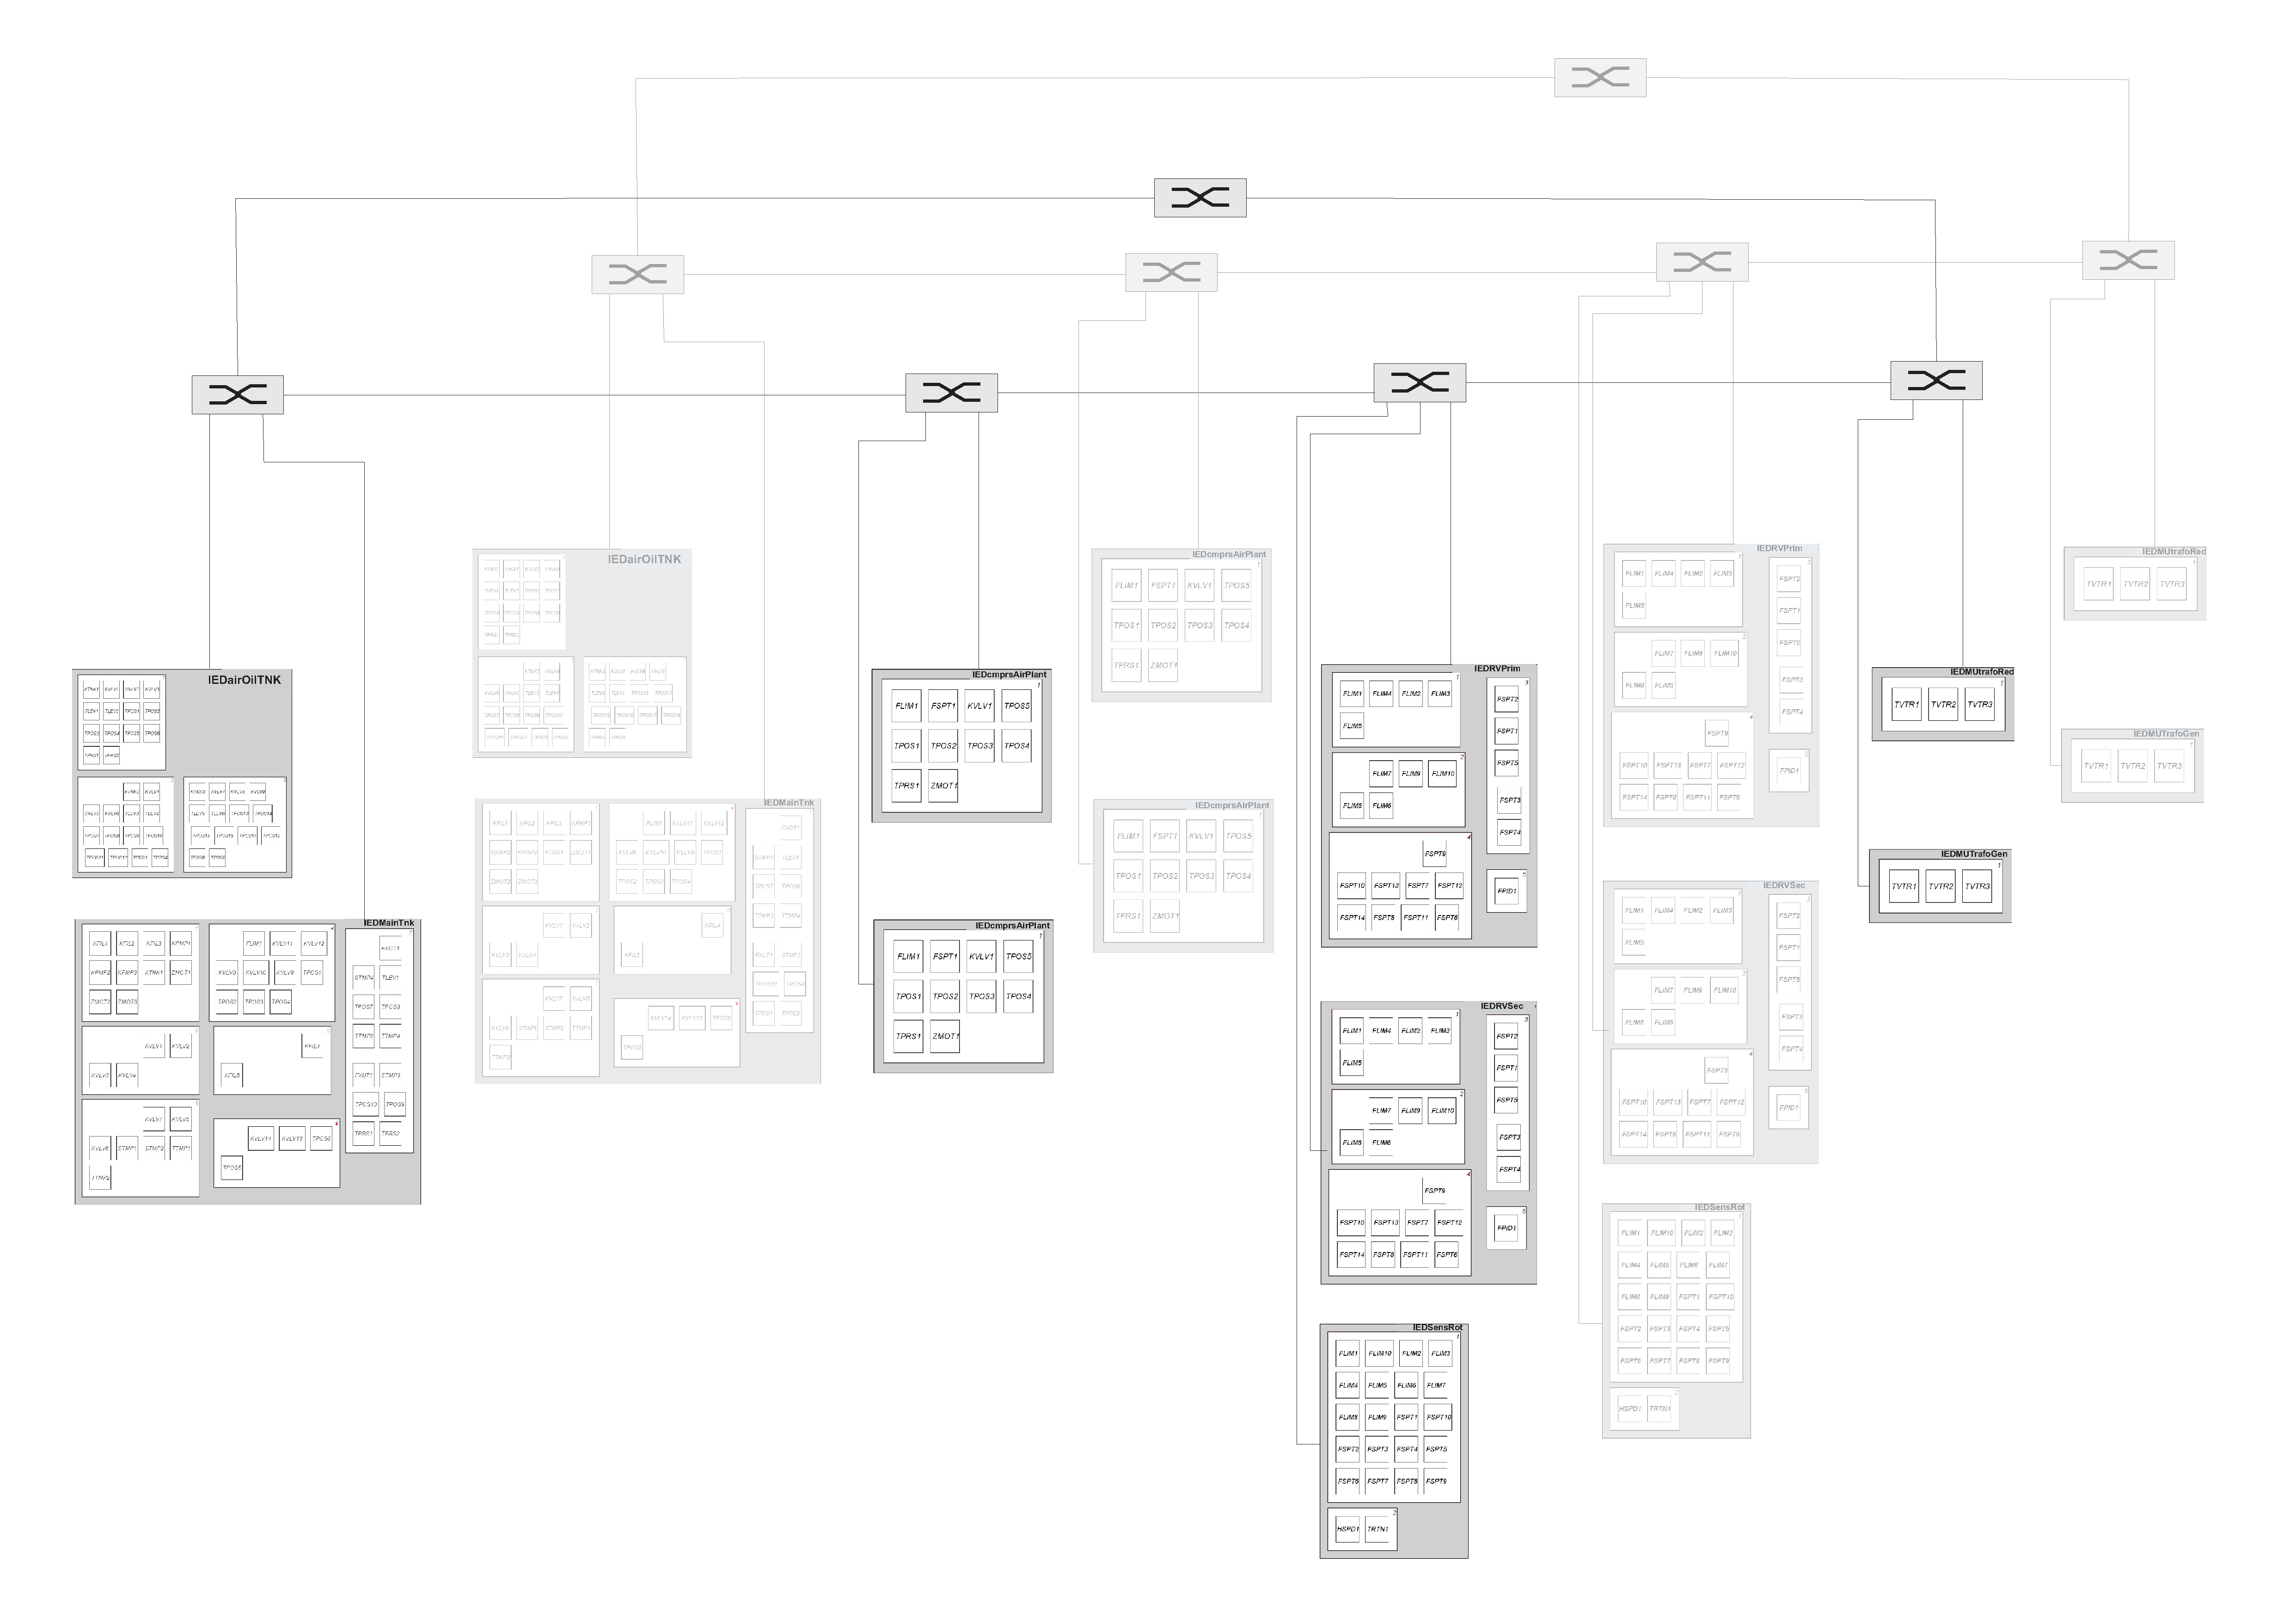
\includegraphics[width=1.0\linewidth]{chapters/model/figures/nodosLogicosDelSistema.eps} 
  \captionsetup{font=scriptsize}
  \caption{Resumen de los nodos l�gicos del regulador de velocidad ubicados seg�n la arquitectura referencial de la figura \ref{fig:arquitectura-Gral-Referencial1} }
  \label{fig:LNodes-reg-veloc}
\end{center}
\end{figure}
\end{landscape}


